\documentclass[tikz,border=8pt]{standalone}
\usepackage[utf8]{inputenc}
\usepackage{amsmath,amssymb}
\usepackage{microtype}
\usetikzlibrary{arrows.meta, calc, positioning,
  decorations.pathmorphing, decorations.markings,
  shapes.geometric, patterns}

\definecolor{deepblue}{RGB}{122, 36, 53}
\definecolor{lightblue}{RGB}{234,215,218}
\definecolor{warmgold}{RGB}{154,106,31}
\definecolor{softgreen}{RGB}{124,95,88}
\definecolor{manifoldcolor}{RGB}{248,232,204}
\definecolor{distcolor}{RGB}{246,235,220}
\definecolor{midblue}{RGB}{138,90,50}

\tikzset{
  >=Stealth,
  mapsto/.style={->, line width=1.3pt, deepblue},
  pullbackarrow/.style={->, line width=1.2pt, warmgold},
  dfstyle/.style={->, line width=0.9pt, midblue, dashed},
  tanvec/.style={->, line width=1.5pt},
  mbox/.style={fill=manifoldcolor, draw=deepblue!40,
               line width=0.8pt, rounded corners=5pt, inner sep=8pt},
  pbox/.style={fill=distcolor, draw=softgreen!50,
               line width=0.8pt, rounded corners=5pt, inner sep=8pt},
}
\begin{document}
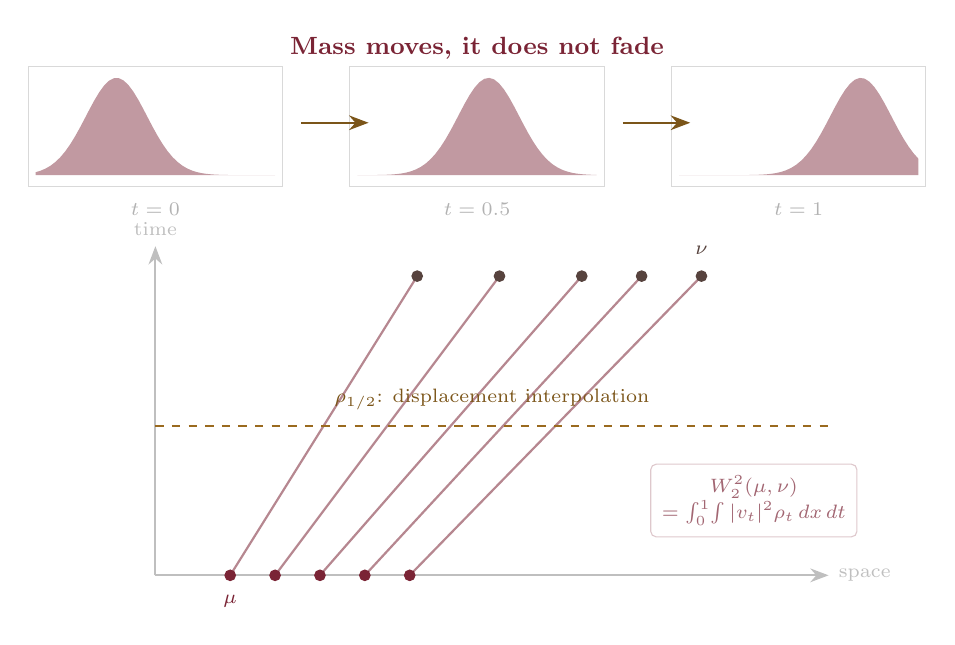
\begin{tikzpicture}[font=\small, scale=0.95]
 
% ---- Top row: density snapshots ----
\foreach \t/\xoff in {0/0, 0.5/4.3, 1/8.6}{
  \begin{scope}[shift={(\xoff,5.3)}]
    \draw[gray!30] (-1.7,-0.1) rectangle (1.7,1.5);
    \pgfmathsetmacro{\mlo}{-1.0+1.5*\t}
    \pgfmathsetmacro{\mhi}{0.6+1.0*\t}
    \fill[deepblue!55,opacity=0.85,domain=-1.6:1.6,samples=50,
          variable=\x]
      plot(\x,{0.05+1.3*exp(-3.0*(\x-(\mlo+0.3*(\mhi-\mlo)))*
                (\x-(\mlo+0.3*(\mhi-\mlo))))})
      -- (1.6,0.05) -- (-1.6,0.05) -- cycle;
    \node[gray!60,font=\scriptsize] at (0,-0.4) {$t=\t$};
  \end{scope}
}
\draw[->,warmgold!80!black,line width=0.9pt] (1.95,6.05) -- (2.85,6.05);
\draw[->,warmgold!80!black,line width=0.9pt] (6.25,6.05) -- (7.15,6.05);
\node[deepblue,font=\small\bfseries] at (4.3,7.05)
  {Mass moves, it does not fade};
 
% ---- Bottom: space-time diagram ----
\begin{scope}[shift={(0,0)}]
  \draw[->,thick,gray!50] (0,0) -- (9.0,0)
    node[right,font=\scriptsize]{space};
  \draw[->,thick,gray!50] (0,0) -- (0,4.4)
    node[above,font=\scriptsize]{time};
 
  \foreach \xs/\xt in {
    1.0/3.5, 1.6/4.6, 2.2/5.7, 2.8/6.5, 3.4/7.3
  }{
    \draw[deepblue!55,thick] (\xs,0) -- (\xt,4.0);
  }
 
  \filldraw[deepblue] (1.0,0) circle (2pt);
  \filldraw[deepblue] (1.6,0) circle (2pt);
  \filldraw[deepblue] (2.2,0) circle (2pt);
  \filldraw[deepblue] (2.8,0) circle (2pt);
  \filldraw[deepblue] (3.4,0) circle (2pt);
 
  \filldraw[softgreen!70!black] (3.5,4.0) circle (2pt);
  \filldraw[softgreen!70!black] (4.6,4.0) circle (2pt);
  \filldraw[softgreen!70!black] (5.7,4.0) circle (2pt);
  \filldraw[softgreen!70!black] (6.5,4.0) circle (2pt);
  \filldraw[softgreen!70!black] (7.3,4.0) circle (2pt);
 
  \node[deepblue,font=\scriptsize] at (1.0,-0.35) {$\mu$};
  \node[softgreen!70!black,font=\scriptsize] at (7.3,4.35) {$\nu$};
 
  \draw[warmgold,dashed,thick] (0,2.0) -- (9.0,2.0)
    node[midway,above=2pt,font=\scriptsize,warmgold!80!black]
      {$\rho_{1/2}$: displacement interpolation};
 
  \node[deepblue!70, font=\scriptsize, align=center,
        draw=deepblue!25, rounded corners=2pt,
        fill=none, inner sep=4pt] at (8.0,1.0)
    {$W_2^2(\mu,\nu)$\\$=\int_0^1\!\int|v_t|^2\rho_t\,dx\,dt$};
\end{scope}
 
\end{tikzpicture}
\end{document}
